%-------------------------------------------------------------------------------
%                                PREAMBLE
%-------------------------------------------------------------------------------
\documentclass[usenames,dvipsnames,svgnames,10pt,aspectratio=169]{beamer}
%
\usefonttheme{professionalfonts}
% This theme uses TIKZ: compile twice with PDFLaTeX or LuaLaTeX.
%
%  Options:
%  - [clean]:    clean slides, i.e. logos and footbar are removed
%  - [kth]:      footbar style inspierd to the official KTH template
%  - [nicewave]: a different style of wave is used (not approved by FLOW)
%
\usetheme[clean]{flow}

\usepackage{tikz}
\usetikzlibrary{arrows}
\usetikzlibrary{shapes.geometric, math, positioning, calc, patterns, angles, quotes}
\usetikzlibrary{patterns.meta,decorations.pathmorphing}

\newcommand{\semaphore}[3]{% #1: color of circle,
                           % #2: color of semicircle
                           % #3: angle of semicircle 
  \tikz[node distance=0mm,baseline]
       {
         \node (s1) [circle, fill=#1, minimum size=6mm] {};
         \node      [semicircle, fill=#2, 
           inner sep=0pt, outer sep=0pt, minimum size=3mm,
           anchor=south,
           at={(s1.center)}, rotate=#3] {};
       }
}

\usepackage[]{circuitikz}

\usepackage{pgfplots}
\usepgfplotslibrary{polar}

\usepackage{hyperref,graphicx,lmodern}
\usepackage[utf8]{inputenc}
\usepackage{media9}
\usepackage{xcolor}
\usepackage{stmaryrd}
\usepackage{nicefrac}
\usepackage{multimedia}
\usepackage{multicol}
\usepackage{upgreek}
\usepackage[]{bm}
\usepackage[]{url}
\usepackage[]{animate}
\usepackage{amsmath}

\usepackage[most]{tcolorbox}

\newcommand*{\TakeFourierOrnament}[1]{{%
    \fontencoding{U}\fontfamily{futs}\selectfont\char#1}}
\newcommand*{\danger}{\TakeFourierOrnament{66}}

\graphicspath{{imgs/}}
\setbeamertemplate{blocks}[rounded][shadow=true]

\DeclareMathOperator*{\maximize}{maximize~}

%-------------------------------------------------------------------------------
%                                TITLE PAGE
%-------------------------------------------------------------------------------
\title[Nonlinear physics] % Short title used in footline
{
  Weakly nonlinear \\ oscillators
}

\author[J.-Ch.~Loiseau] % Presenting author in short form used in footline
{
	\underline{Jean-Christophe Loiseau}
}
% - Give the names in the same order as the appear in the paper.
% - Underline the presenting author.

\institute[unused]
{
	\url{jean-christophe.loiseau@ensam.eu} \\
	Laboratoire DynFluid \\
	Arts et M\'etiers, France.
}
% Keep it simple, no one is interested in your street address.

% University logo(s)
\logot{
\includegraphics[width=.128\paperwidth]{DynFluid_logo}}  % Top logo
\logob{
\includegraphics[width=0.128\paperwidth]{ENSAM_logo}} % Bottom logo
% \logoc[{\includegraphics[width=.128\paperwidth]{limsi}}]{\includegraphics[width=.128\paperwidth]{limsi}} % Corner logo
%
% Cover image: \cvrimg{x position}{y position}{cover image}
\cvrimg{.77}{.8}{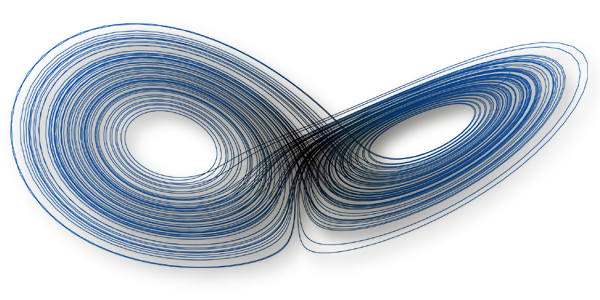
\includegraphics[width=.4\paperwidth]{cover.png}}

\date[unused]{Physique non-lin\'eaire -- 2019-2020}

\begin{document}

\titleframe	% Print the title as the first slide

%-------------------------------------------------------------------------------
%                           PRESENTATION SLIDES
%-------------------------------------------------------------------------------

\begin{frame}[t, c]{Weakly nonlinear oscillators}{Multiple time scales}
  \begin{minipage}{.68\textwidth}
    \[
    \tcboxmath[colframe=beamer@kthblue, colback=white]{
      \ddot{x} + x + \epsilon h(x, \dot{x}) = 0
    }
    \]

    \bigskip

    Nonlinear oscillators are often characterized by dynamics at different time scales, e.g. the phase tends to change at a faster rate than the oscillation's amplitude.

  \end{minipage}%
  \hfill
  \begin{minipage}{.28\textwidth}
    \centering
    \begin{tikzpicture}[>=stealth]
      \draw[->] (-2, 0) -- (2, 0) node[below] {$x$};
      \draw[->] (0, -2) -- (0, 2) node[left] {$\dot{x}$};
      
      \draw[gray, thick] plot file{van_der_pol_traj_bis.txt};
      
      \node[circle, fill=white, draw=black, inner sep=0pt, minimum size=4pt] at (0, 0) {};
    \end{tikzpicture}
  \end{minipage}
\end{frame}

\begin{frame}[t, c]{Weakly nonlinear oscillators}{Examples : the van der Pol oscillator}
  \begin{minipage}{.68\textwidth}
    \[
    \tcboxmath[colframe=beamer@kthblue, colback=white]{
      \begin{aligned}
        \textbf{van der Pol osc.\ :} \quad & \ddot{x} + x + \epsilon \left( x^2 - 1 \right) \dot{x} = 0 \\
        & x(0) = 1, \quad \dot{x}(0) = 0
      \end{aligned}
    }
    \]
    
    \bigskip

    It is a canonical example of nonlinear oscillators proposed in 1927 by the Dutch electrical engineer Balthasar van der Pol.
  \end{minipage}%
  \hfill
  \begin{minipage}{.28\textwidth}
    \centering
    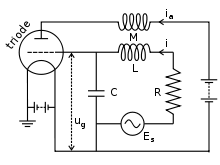
\includegraphics[width=\textwidth]{van_der_pol}
  \end{minipage}
\end{frame}

\begin{frame}[t, c]{Weakly nonlinear oscillators}{Example : van der Pol oscillator}
  \textbf{Fast time scale :} $\tau = t$ for the evolution of the phase.

  \medskip

  \textbf{Slow time scale :} $T = \epsilon t$ for the evolution of the oscillation's amplitude.

  \medskip

  \textbf{Power series expansion :} $x(t, \epsilon) = x_0(\tau, T) + \epsilon x_1(\tau, T) + \mathcal{O}(\epsilon^2)$

  \bigskip

  \[
  \tcboxmath[colframe=beamer@kthblue, colback=white]{
    \begin{aligned}
      \mathcal{O}(1) : \quad & \dfrac{\partial^2 x_0}{\partial \tau^2} + x_0 = 0 \\
      \mathcal{O}(\epsilon) : \quad & \dfrac{\partial^2 x_1}{\partial \tau^2} + x_1 = - 2\dfrac{\partial^2 x_0}{\partial \tau \partial T} - \left( x_0^2 - 1 \right) \dfrac{\partial x_0}{\partial \tau}
    \end{aligned}
  }
  \]
\end{frame}




\begin{frame}[t, c]{Weakly nonlinear oscillators}{Example : van der Pol oscillator}
  \[
  \tcboxmath[colframe=beamer@kthblue, colback=white]{
    \mathcal{O}(1) : \quad \dfrac{\partial^2 x_0}{\partial \tau^2} + x_0 = 0
  }
  \]

  \bigskip

  As usual, the dynamics at order zero are captured by a simple harmonic oscillator.
  The general solution can be written as
  %
  \[
  x_0(\tau, T) = r(T) \cos\left( \tau + \varphi(T) \right)
  \]
  %
  where $r(T)$ and $\varphi(T)$ are the \alert{\textbf{slowly varying amplitude and phase}} of $x_0$.
\end{frame}





\begin{frame}[t, c]{Weakly nonlinear oscillators}{Example : van der Pol oscillator}
  \[
  \tcboxmath[colback=white, colframe=beamer@kthblue]{
    \mathcal{O}(\epsilon) : \quad \dfrac{\partial^2 x_1}{\partial \tau^2} + x_1 = -2 \left( \dot{r} \sin(\tau + \varphi) + r \dot{\varphi} \cos(\tau + \varphi) \right) - r \sin(\tau + \varphi) \left( r^2 \cos^2(\tau + \varphi) - 1 \right)
  }
  \]

  \bigskip

  {\Large \danger} The right-hand side contains \alert{\textbf{resonant}} terms which would leads to unphysical \alert{\textbf{secular growth}}.
  %
  \[
  \textbf{Trig.\ identity :} \quad \sin(\tau + \varphi) \cos^2(\tau + \varphi) = \dfrac{1}{4} \left( \sin(\tau + \varphi \right) + \sin\left( 3(\tau + \varphi) \right)
  \]
\end{frame}




\begin{frame}[t, c]{Weakly nonlinear oscillators}{Example : van der Pol oscillator}
  \[
  \tcboxmath[colback=white, colframe=beamer@kthblue]{
    \mathcal{O}(\epsilon) : \quad \dfrac{\partial^2 x_1}{\partial \tau^2} + x_1 = \left( -2 \dot{r} + r - \dfrac{r^3}{4} \right) \sin(\tau + \varphi) - 2 r \dot{\varphi} \cos(\tau + \varphi) - \dfrac{r^3}{4} \sin\left( 3(\tau + \varphi) \right)
  }
  \]

  \bigskip

  The slowly varying amplitude and phase $r(T)$ and $\varphi(T)$ need to satisfy
  %
  \[
  \dfrac{dr}{dT} = \dfrac{1}{8} r \left( 4 - r^2 \right), \quad \text{and} \quad \dfrac{d \varphi}{dT} = 0
  \]
  %
  to avoid \alert{\textbf{secular growth}}.

\end{frame}




\begin{frame}[t, c]{Weakly nonlinear oscillators}{Example : van der Pol oscillator}
  \begin{minipage}{.58\textwidth}
    The slowly-varying amplitude obeys
    %
    \[
    \dfrac{dr}{dt} = \dfrac{\epsilon}{8} r \left( 4 - r^2 \right).
    \]
    %
    It has two fixed points : $r^* = 0$ is linearly unstable while $r^* = 2$ is linearly stable.
    Hence, as $t \to \infty$, $r(t) \to 2$.
  \end{minipage}%
  \hfill
  \begin{minipage}{.38\textwidth}
    \centering
    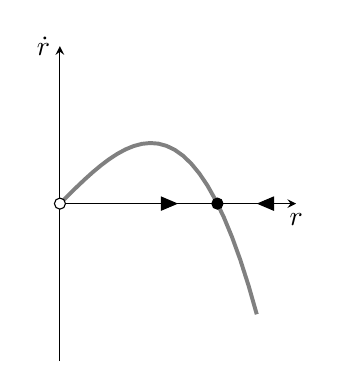
\begin{tikzpicture}[>=stealth]
      \draw[->] (0, 0) -- (3, 0) node[below] {$r$};
      \draw[->] (0, -2) -- (0, 2) node[left] {$\dot{r}$};
      
      \draw[gray, line width=0.5mm, domain=0:2.5] plot (\x, {(1/4) * \x * ( 4 - \x * \x)});
      
      \node[rotate=-90, inner sep=0pt] () at (1.5, 0) {\tikz\draw[-triangle 45](0, 0) ;};
      \node[circle, fill=white, draw=black, inner sep=0pt, minimum size=4pt] (a) at (0, 0) {};


      \node[rotate=90, inner sep=0pt] () at (2.5, 0) {\tikz\draw[-triangle 45](0, 0) ;};
      \node[circle, fill=black, draw=black, inner sep=0pt, minimum size=4pt] (a) at (2, 0) {};
    \end{tikzpicture}
  \end{minipage}
\end{frame}

\begin{frame}[t, c]{Weakly nonlinear oscillators}{Example : van der Pol oscillator}
  \centering

  \[
  \tcboxmath[colback=white, colframe=beamer@kthblue]{
    \begin{aligned}
      \textbf{Two-timing :} & \quad x(t) = r(t) \cos( t + \varphi_0 ) \\
      \text{with} & \quad \lim_{t \to \infty} r(t) = 2 \ \text{for $\epsilon > 0$}
    \end{aligned}
  }
  \]

  \bigskip

  \begin{tikzpicture}[>=stealth]
    \draw[->, thick] (-1, 0) -- (11, 0) node[below] {$t$};
    \draw[->, thick] (0, -1.75) -- (0, 1.75) node[left] {$x$};

    \draw[gray, thick] plot file{traj_x.txt};
    \draw[beamer@kthblue, thick] plot file{traj_r.txt};

  \end{tikzpicture}

  \vspace{1cm}
\end{frame}


\end{document}
